\documentclass{article} % For LaTeX2e
\usepackage{graphicx}
\usepackage{caption}
\usepackage{subcaption}
\usepackage{amssymb}
\usepackage{amsmath}
\usepackage{nips14submit_e,times}
\usepackage{hyperref}
\usepackage{url}
\usepackage{verbatim}
%\usepackage{natbib}
%\documentstyle[nips14submit_09,times,art10]{article} % For LaTeX 2.09

\DeclareMathOperator{\x}{\mathbf{x}}
\DeclareMathOperator{\e}{\mathbf{e}}
\DeclareMathOperator{\M}{\mathbf{M}}
\DeclareMathOperator{\w}{\mathbf{w}}
\newcommand{\fix}{\marginpar{FIX}}
\newcommand{\new}{\marginpar{NEW}}
\edef\polishl{\l} 



\RequirePackage{latexsym}
\RequirePackage{amsmath}
\RequirePackage{amssymb} 
\RequirePackage{color} 
\RequirePackage{bm}
\RequirePackage{color}
\RequirePackage{picinpar}

%%%%%%%% Stock standard definitions %%%%%%%%%%%%%%%

\newcommand{\wbt}{\widetilde{\mathbf{w}}}
\DeclareMathOperator{\ab}{\mathbf{a}}
\DeclareMathOperator{\abh}{\widehat{\ab}}
\DeclareMathOperator{\bb}{\mathbf{b}}
\DeclareMathOperator{\bbh}{\widehat{\bb}}
\DeclareMathOperator{\cb}{\mathbf{c}}
\DeclareMathOperator{\db}{\mathbf{d}}
\DeclareMathOperator{\eb}{\mathbf{e}}
\DeclareMathOperator{\fb}{\mathbf{f}}
\DeclareMathOperator{\gb}{\mathbf{g}}
\DeclareMathOperator{\hb}{\mathbf{h}}
\DeclareMathOperator{\ib}{\mathbf{i}}
\DeclareMathOperator{\jb}{\mathbf{j}}
\DeclareMathOperator{\kb}{\mathbf{k}}
\DeclareMathOperator{\lb}{\mathbf{l}}
\DeclareMathOperator{\mb}{\mathbf{m}}
\DeclareMathOperator{\nbb}{\mathbf{n}}
\DeclareMathOperator{\ob}{\mathbf{o}}
\DeclareMathOperator{\pb}{\mathbf{p}}
\DeclareMathOperator{\qb}{\mathbf{q}}
\DeclareMathOperator{\rb}{\mathbf{r}}
\DeclareMathOperator{\sbb}{\mathbf{s}}
\DeclareMathOperator{\tb}{\mathbf{t}}
\DeclareMathOperator{\ub}{\mathbf{u}}
\DeclareMathOperator{\vb}{\mathbf{v}}
\DeclareMathOperator{\wb}{\mathbf{w}}
\DeclareMathOperator{\xb}{\mathbf{x}}
\DeclareMathOperator{\yb}{\mathbf{y}}
\DeclareMathOperator{\zb}{\mathbf{z}}
\renewcommand{\l}{\ell}

\DeclareMathOperator{\atilde}{\tilde{\ab}}
\DeclareMathOperator{\btilde}{\tilde{\bb}}
\DeclareMathOperator{\ctilde}{\tilde{\cb}}
\DeclareMathOperator{\dtilde}{\tilde{\db}}
\DeclareMathOperator{\etilde}{\tilde{\eb}}
\DeclareMathOperator{\ftilde}{\tilde{\fb}}
\DeclareMathOperator{\gtilde}{\tilde{\gb}}
\DeclareMathOperator{\htilde}{\tilde{\hb}}
\DeclareMathOperator{\itilde}{\tilde{\ib}}
\DeclareMathOperator{\jtilde}{\tilde{\jb}}
\DeclareMathOperator{\ktilde}{\tilde{\kb}}
\DeclareMathOperator{\ltilde}{\tilde{\lb}}
\DeclareMathOperator{\mtilde}{\tilde{\mb}}
\DeclareMathOperator{\ntilde}{\tilde{\nbb}}
\DeclareMathOperator{\otilde}{\tilde{\ob}}
\DeclareMathOperator{\ptilde}{\tilde{\pb}}
\DeclareMathOperator{\qtilde}{\tilde{\qb}}
\DeclareMathOperator{\rtilde}{\tilde{\rb}}
\DeclareMathOperator{\stilde}{\tilde{\sbb}}
\DeclareMathOperator{\ttilde}{\tilde{\tb}}
\DeclareMathOperator{\utilde}{\tilde{\ub}}
\DeclareMathOperator{\vtilde}{\tilde{\vb}}
\DeclareMathOperator{\wtilde}{\tilde{\wb}}
\DeclareMathOperator{\xtilde}{\tilde{\xb}}
\DeclareMathOperator{\ytilde}{\tilde{\yb}}
\DeclareMathOperator{\ztilde}{\tilde{\zb}}

\DeclareMathOperator{\abar}{\bar{\ab}}
\DeclareMathOperator{\bbar}{\bar{\bb}}
\DeclareMathOperator{\cbar}{\bar{\cb}}
\DeclareMathOperator{\dbar}{\bar{\db}}
\DeclareMathOperator{\ebar}{\bar{\eb}}
\DeclareMathOperator{\fbar}{\bar{\fb}}
\DeclareMathOperator{\gbar}{\bar{\gb}}
\DeclareMathOperator{\hbbar}{\bar{\hb}}
\DeclareMathOperator{\ibar}{\bar{\ib}}
\DeclareMathOperator{\jbar}{\bar{\jb}}
\DeclareMathOperator{\kbar}{\bar{\kb}}
\DeclareMathOperator{\lbar}{\bar{\lb}}
\DeclareMathOperator{\mbar}{\bar{\mb}}
\DeclareMathOperator{\nbar}{\bar{\nbb}}
\DeclareMathOperator{\obar}{\bar{\ob}}
\DeclareMathOperator{\pbar}{\bar{\pb}}
\DeclareMathOperator{\qbar}{\bar{\qb}}
\DeclareMathOperator{\rbar}{\bar{\rb}}
\DeclareMathOperator{\sbar}{\bar{\sbb}}
\DeclareMathOperator{\tbar}{\bar{\tb}}
\DeclareMathOperator{\ubar}{\bar{\ub}}
\DeclareMathOperator{\vbar}{\bar{\vb}}
\DeclareMathOperator{\wbar}{\bar{\wb}}
\DeclareMathOperator{\xbar}{\bar{\xb}}
\DeclareMathOperator{\ybar}{\bar{\yb}}
\DeclareMathOperator{\zbar}{\bar{\zb}}

\DeclareMathOperator{\Ab}{\mathbf{A}}
\DeclareMathOperator{\Bb}{\mathbf{B}}
\DeclareMathOperator{\Cb}{\mathbf{C}}
\DeclareMathOperator{\Db}{\mathbf{D}}
\DeclareMathOperator{\Eb}{\mathbf{E}}
\DeclareMathOperator{\Fb}{\mathbf{F}}
\DeclareMathOperator{\Gb}{\mathbf{G}}
\DeclareMathOperator{\Hb}{\mathbf{H}}
\DeclareMathOperator{\Ib}{\mathbf{I}}
\DeclareMathOperator{\Jb}{\mathbf{J}}
\DeclareMathOperator{\Kb}{\mathbf{K}}
\DeclareMathOperator{\Lb}{\mathbf{L}}
\DeclareMathOperator{\Mb}{\mathbf{M}}
\DeclareMathOperator{\Nb}{\mathbf{N}}
\DeclareMathOperator{\Ob}{\mathbf{O}}
\DeclareMathOperator{\Pb}{\mathbf{P}}
\DeclareMathOperator{\Qb}{\mathbf{Q}}
\DeclareMathOperator{\Rb}{\mathbf{R}}
\DeclareMathOperator{\Sbb}{\mathbf{S}}
\DeclareMathOperator{\Tb}{\mathbf{T}}
\DeclareMathOperator{\Ub}{\mathbf{U}}
\DeclareMathOperator{\Vb}{\mathbf{V}}
\DeclareMathOperator{\Wb}{\mathbf{W}}
\DeclareMathOperator{\Xb}{\mathbf{X}}
\DeclareMathOperator{\Xbt}{\widetilde{\Xb}}
\DeclareMathOperator{\Xbh}{\widehat{\Xb}}
\DeclareMathOperator{\Xbs}{\widetilde{\Xb}}
\DeclareMathOperator{\Zbs}{\widetilde{\Zb}}
\DeclareMathOperator{\Kbs}{\widetilde{\Kb}}
\DeclareMathOperator{\Zbh}{\widehat{\Zb}}
\DeclareMathOperator{\Ubh}{\widehat{\Ub}}
\DeclareMathOperator{\Yb}{\mathbf{Y}}
\DeclareMathOperator{\Zb}{\mathbf{Z}}

\DeclareMathOperator{\Abar}{\bar{A}}
\DeclareMathOperator{\Bbar}{\bar{B}}
\DeclareMathOperator{\Cbar}{\bar{C}}
\DeclareMathOperator{\Dbar}{\bar{D}}
\DeclareMathOperator{\Ebar}{\bar{E}}
\DeclareMathOperator{\Fbar}{\bar{F}}
\DeclareMathOperator{\Gbar}{\bar{G}}
\DeclareMathOperator{\Hbar}{\bar{H}}
\DeclareMathOperator{\Ibar}{\bar{I}}
\DeclareMathOperator{\Jbar}{\bar{J}}
\DeclareMathOperator{\Kbar}{\bar{K}}
\DeclareMathOperator{\Lbar}{\bar{L}}
\DeclareMathOperator{\Mbar}{\bar{M}}
\DeclareMathOperator{\Nbar}{\bar{N}}
\DeclareMathOperator{\Obar}{\bar{O}}
\DeclareMathOperator{\Pbar}{\bar{P}}
\DeclareMathOperator{\Qbar}{\bar{Q}}
\DeclareMathOperator{\Rbar}{\bar{R}}
\DeclareMathOperator{\Sbar}{\bar{S}}
\DeclareMathOperator{\Tbar}{\bar{T}}
\DeclareMathOperator{\Ubar}{\bar{U}}
\DeclareMathOperator{\Vbar}{\bar{V}}
\DeclareMathOperator{\Wbar}{\bar{W}}
\DeclareMathOperator{\Xbar}{\bar{X}}
\DeclareMathOperator{\Ybar}{\bar{Y}}
\DeclareMathOperator{\Zbar}{\bar{Z}}

\DeclareMathOperator{\Abbar}{\bar{\Ab}}
\DeclareMathOperator{\Bbbar}{\bar{\Bb}}
\DeclareMathOperator{\Cbbar}{\bar{\Cb}}
\DeclareMathOperator{\Dbbar}{\bar{\Db}}
\DeclareMathOperator{\Ebbar}{\bar{\Eb}}
\DeclareMathOperator{\Fbbar}{\bar{\Fb}}
\DeclareMathOperator{\Gbbar}{\bar{\Gb}}
\DeclareMathOperator{\Hbbar}{\bar{\Hb}}
\DeclareMathOperator{\Ibbar}{\bar{\Ib}}
\DeclareMathOperator{\Jbbar}{\bar{\Jb}}
\DeclareMathOperator{\Kbbar}{\bar{\Kb}}
\DeclareMathOperator{\Lbbar}{\bar{\Lb}}
\DeclareMathOperator{\Mbbar}{\bar{\Mb}}
\DeclareMathOperator{\Nbbar}{\bar{\Nb}}
\DeclareMathOperator{\Obbar}{\bar{\Ob}}
\DeclareMathOperator{\Pbbar}{\bar{\Pb}}
\DeclareMathOperator{\Qbbar}{\bar{\Qb}}
\DeclareMathOperator{\Rbbar}{\bar{\Rb}}
\DeclareMathOperator{\Sbbar}{\bar{\Sb}}
\DeclareMathOperator{\Tbbar}{\bar{\Tb}}
\DeclareMathOperator{\Ubbar}{\bar{\Ub}}
\DeclareMathOperator{\Vbbar}{\bar{\Vb}}
\DeclareMathOperator{\Wbbar}{\bar{\Wb}}
\DeclareMathOperator{\Xbbar}{\bar{\Xb}}
\DeclareMathOperator{\Ybbar}{\bar{\Yb}}
\DeclareMathOperator{\Zbbar}{\bar{\Zb}}

\DeclareMathOperator{\Ahat}{\widehat{A}}
\DeclareMathOperator{\Bhat}{\widehat{B}}
\DeclareMathOperator{\Chat}{\widehat{C}}
\DeclareMathOperator{\Dhat}{\widehat{D}}
\DeclareMathOperator{\Ehat}{\widehat{E}}
\DeclareMathOperator{\Fhat}{\widehat{F}}
\DeclareMathOperator{\Ghat}{\widehat{G}}
\DeclareMathOperator{\Hhat}{\widehat{H}}
\DeclareMathOperator{\Ihat}{\widehat{I}}
\DeclareMathOperator{\Jhat}{\widehat{J}}
\DeclareMathOperator{\Khat}{\widehat{K}}
\DeclareMathOperator{\Lhat}{\widehat{L}}
\DeclareMathOperator{\Mhat}{\widehat{M}}
\DeclareMathOperator{\Nhat}{\widehat{N}}
\DeclareMathOperator{\Ohat}{\widehat{O}}
\DeclareMathOperator{\Phat}{\widehat{P}}
\DeclareMathOperator{\Qhat}{\widehat{Q}}
\DeclareMathOperator{\Rhat}{\widehat{R}}
\DeclareMathOperator{\Shat}{\widehat{S}}
\DeclareMathOperator{\That}{\widehat{T}}
\DeclareMathOperator{\Uhat}{\widehat{U}}
\DeclareMathOperator{\Vhat}{\widehat{V}}
\DeclareMathOperator{\What}{\widehat{W}}
\DeclareMathOperator{\Xhat}{\widehat{X}}
\DeclareMathOperator{\Yhat}{\widehat{Y}}
\DeclareMathOperator{\Zhat}{\widehat{Z}}

\DeclareMathOperator{\Abhat}{\widehat{\Ab}}
\DeclareMathOperator{\Bbhat}{\widehat{\Bb}}
\DeclareMathOperator{\Cbhat}{\widehat{\Cb}}
\DeclareMathOperator{\Dbhat}{\widehat{\Db}}
\DeclareMathOperator{\Ebhat}{\widehat{\Eb}}
\DeclareMathOperator{\Fbhat}{\widehat{\Fb}}
\DeclareMathOperator{\Gbhat}{\widehat{\Gb}}
\DeclareMathOperator{\Hbhat}{\widehat{\Hb}}
\DeclareMathOperator{\Ibhat}{\widehat{\Ib}}
\DeclareMathOperator{\Jbhat}{\widehat{\Jb}}
\DeclareMathOperator{\Kbhat}{\widehat{\Kb}}
\DeclareMathOperator{\Lbhat}{\widehat{\Lb}}
\DeclareMathOperator{\Mbhat}{\widehat{\Mb}}
\DeclareMathOperator{\Nbhat}{\widehat{\Nb}}
\DeclareMathOperator{\Obhat}{\widehat{\Ob}}
\DeclareMathOperator{\Pbhat}{\widehat{\Pb}}
\DeclareMathOperator{\Qbhat}{\widehat{\Qb}}
\DeclareMathOperator{\Rbhat}{\widehat{\Rb}}
\DeclareMathOperator{\Sbhat}{\widehat{\Sb}}
\DeclareMathOperator{\Tbhat}{\widehat{\Tb}}
\DeclareMathOperator{\Ubhat}{\widehat{\Ub}}
\DeclareMathOperator{\Vbhat}{\widehat{\Vb}}
\DeclareMathOperator{\Wbhat}{\widehat{\Wb}}
\DeclareMathOperator{\Xbhat}{\widehat{\Xb}}
\DeclareMathOperator{\Ybhat}{\widehat{\Yb}}
\DeclareMathOperator{\Zbhat}{\widehat{\Zb}}

\DeclareMathOperator{\Acal}{\mathcal{A}}
\DeclareMathOperator{\Bcal}{\mathcal{B}}
\DeclareMathOperator{\Ccal}{\mathcal{C}}
\DeclareMathOperator{\Dcal}{\mathcal{D}}
\DeclareMathOperator{\Ecal}{\mathcal{E}}
\DeclareMathOperator{\Fcal}{\mathcal{F}}
\DeclareMathOperator{\Gcal}{\mathcal{G}}
\DeclareMathOperator{\Hcal}{\mathcal{H}}
\DeclareMathOperator{\Ical}{\mathcal{I}}
\DeclareMathOperator{\Jcal}{\mathcal{J}}
\DeclareMathOperator{\Kcal}{\mathcal{K}}
\DeclareMathOperator{\Lcal}{\mathcal{L}}
\DeclareMathOperator{\Mcal}{\mathcal{M}}
\DeclareMathOperator{\Ncal}{\mathcal{N}}
\DeclareMathOperator{\Ocal}{\mathcal{O}}
\DeclareMathOperator{\Pcal}{\mathcal{P}}
\DeclareMathOperator{\Qcal}{\mathcal{Q}}
\DeclareMathOperator{\Rcal}{\mathcal{R}}
\DeclareMathOperator{\Scal}{\mathcal{S}}
\DeclareMathOperator{\Scalt}{\widetilde{\Scal}}
\DeclareMathOperator{\Tcal}{\mathcal{T}}
\DeclareMathOperator{\Ucal}{\mathcal{U}}
\DeclareMathOperator{\Vcal}{\mathcal{V}}
\DeclareMathOperator{\Wcal}{\mathcal{W}}
\DeclareMathOperator{\Xcal}{\mathcal{X}}
\DeclareMathOperator{\Ycal}{\mathcal{Y}}
\DeclareMathOperator{\Zcal}{\mathcal{Z}}

\DeclareMathOperator{\Atilde}{\widetilde{A}}
\DeclareMathOperator{\Btilde}{\widetilde{B}}
\DeclareMathOperator{\Ctilde}{\widetilde{C}}
\DeclareMathOperator{\Dtilde}{\widetilde{D}}
\DeclareMathOperator{\Etilde}{\widetilde{E}}
\DeclareMathOperator{\Ftilde}{\widetilde{F}}
\DeclareMathOperator{\Gtilde}{\widetilde{G}}
\DeclareMathOperator{\Htilde}{\widetilde{H}}
\DeclareMathOperator{\Itilde}{\widetilde{I}}
\DeclareMathOperator{\Jtilde}{\widetilde{J}}
\DeclareMathOperator{\Ktilde}{\widetilde{K}}
\DeclareMathOperator{\Ltilde}{\widetilde{L}}
\DeclareMathOperator{\Mtilde}{\widetilde{M}}
\DeclareMathOperator{\Ntilde}{\widetilde{N}}
\DeclareMathOperator{\Otilde}{\widetilde{O}}
\DeclareMathOperator{\Ptilde}{\widetilde{P}}
\DeclareMathOperator{\Qtilde}{\widetilde{Q}}
\DeclareMathOperator{\Rtilde}{\widetilde{R}}
\DeclareMathOperator{\Stilde}{\widetilde{S}}
\DeclareMathOperator{\Ttilde}{\widetilde{T}}
\DeclareMathOperator{\Utilde}{\widetilde{U}}
\DeclareMathOperator{\Vtilde}{\widetilde{V}}
\DeclareMathOperator{\Wtilde}{\widetilde{W}}
\DeclareMathOperator{\Xtilde}{\widetilde{X}}
\DeclareMathOperator{\Ytilde}{\widetilde{Y}}
\DeclareMathOperator{\Ztilde}{\widetilde{Z}}


%%%%%%%% Widely accepted definitions %%%%%%%%%%%%%%%

\DeclareMathOperator{\CC}{\mathbb{C}} % Complex numbers
\DeclareMathOperator{\EE}{\mathbb{E}} % Expectation
\DeclareMathOperator{\KK}{\mathbb{K}} % Arbitrary field
\DeclareMathOperator{\MM}{\mathbb{M}} % Median
\DeclareMathOperator{\NN}{\mathbb{N}} % Natural numbers
\DeclareMathOperator{\PP}{\mathbb{P}} % Probability
\DeclareMathOperator{\QQ}{\mathbb{Q}} % Rationals
\DeclareMathOperator{\RR}{\mathbb{R}} % Real numbers 
\DeclareMathOperator{\ZZ}{\mathbb{Z}} % Integers

\DeclareMathOperator{\one}{\mathbf{1}}  % Identity
\DeclareMathOperator{\zero}{\mathbf{0}} % Zero
\DeclareMathOperator{\TRUE}{\mathbf{TRUE}}  % True
\DeclareMathOperator{\FALSE}{\mathbf{FALSE}}  % False

\DeclareMathOperator*{\mini}{\mathop{\mathrm{minimize}}}
\DeclareMathOperator*{\maxi}{\mathop{\mathrm{maximize}}}
\DeclareMathOperator*{\argmin}{\mathop{\mathrm{argmin}}}
\DeclareMathOperator*{\argmax}{\mathop{\mathrm{argmax}}}
\DeclareMathOperator*{\argsup}{\mathop{\mathrm{argsup}}}
\DeclareMathOperator*{\arginf}{\mathop{\mathrm{arginf}}}
\DeclareMathOperator{\sgn}{\mathop{\mathrm{sign}}}
\DeclareMathOperator{\sign}{\mathop{\mathrm{sign}}}
\DeclareMathOperator{\tr}{\mathop{\mathrm{tr}}}
\DeclareMathOperator{\rank}{\mathop{\mathrm{rank}}}
\DeclareMathOperator{\traj}{\mathop{\mathrm{Traj}}}

%%%%%%%% Bold Greek Letters %%%%%%%%%%%%%%%
\DeclareMathOperator{\sigmab}{\bm{\sigma}}
\DeclareMathOperator{\Sigmab}{\mathbf{\Sigma}}


%%%%%%%% Mess around with LaTeX %%%%%%%%%%%%%%%

%% Some style files might actually define these variables.
%% So don't mess with them if they are already defined

\ifx\BlackBox\undefined
\newcommand{\BlackBox}{\rule{1.5ex}{1.5ex}}  % end of proof
\fi

\ifx\proof\undefined
\newenvironment{proof}{\par\noindent{\bf Proof\ }}{\hfill\BlackBox\\[2mm]}
% \else
% \renewenvironment{proof}{\par\noindent{\bf Proof\ }}{\hfill\BlackBox\\[2mm]}
\fi

%Trying to put all on Section track
%\makeatletter
%\@addtoreset{equation}{section}
%\def\theequation{\thesection.\arabic{equation}}
%\def\thetheorem{\thesection.\arabic{theorem}}
%\makeatother

%the below clashes with the previous defs of them... 
%in the style files
%\newtheorem{theorem}{Theorem}[section]
%\newtheorem{lemma}[theorem]{Lemma}
%\newtheorem{corollary}[theorem]{Corollary}
%\newtheorem{conjecture}[conjecture]{Conjecture}


%%%%%%%% Utility functions %%%%%%%%%%%%%%%

\newcommand{\eq}[1]{(\ref{#1})} 
\newcommand{\mymatrix}[2]{\left[\begin{array}{#1} #2 \end{array}\right]}
\newcommand{\mychoose}[2]{\left(\begin{array}{c} #1 \\ #2 \end{array}\right)}
\newcommand{\mydet}[1]{\det\left[ #1 \right]}
\newcommand{\sembrack}[1]{[\![#1]\!]}

\newcommand{\ea}{\emph{et al. }}
\newcommand{\eg}{\emph{e.g. }}
\newcommand{\ie}{\emph{i.e., }}

\newcommand{\mnote}[1]{\marginpar{#1}}
\newcommand{\note}[1]{{\bf {#1}}}

%%%%%%%% Specific symbols for this project %%%%%%%%%%%%%%%

\DeclareMathOperator{\half}{\frac{1}{2}}

\newcommand{\Ref}[1]{\hfill\Green{[#1]}}
\DeclareMathOperator{\XX}{\mathcal{X}}
\newcommand{\ar}{\implies}
\newcommand{\yh}{\hat{y}}
\DeclareMathOperator{\lan}{\langle}
\DeclareMathOperator{\ran}{\rangle}

\DeclareMathOperator{\dc}{\mathrm{dc}}

\DeclareMathOperator{\Utb}{\widetilde{\Ub}}
\DeclareMathOperator{\Stb}{\widetilde{\Sbb}}

\ifx\Brown\undefined
\definecolor{brown}{rgb}{0.5,0.1,0.1}
\newcommand{\Brown}[1]{\color{brown}{#1}\color{black}}
\fi

\ifx\Red\undefined
\definecolor{red}{rgb}{1.0,0,0}
\newcommand{\Red}[1]{\color{red}{#1}\color{black}}
\fi

\ifx\Green\undefined
\definecolor{green}{rgb}{0,0.4,0}
\newcommand{\Green}[1]{\color{green}{#1}\color{black}}
\fi

\ifx\Blue\undefined
\definecolor{blue}{rgb}{0,0,1.0}
\newcommand{\Blue}[1]{\color{blue}{#1}\color{black}}
\fi



\newcommand{\beq}{\begin{equation}}
\newcommand{\eeq}{\end{equation}}
\newcommand{\beh}{\begin{conjecture}}
\newcommand{\eeh}{\end{conjecture}}
\newcommand\bel{\begin{lemma}}
\newcommand\eel{\end{lemma}}
\newcommand\bet{\begin{theoreme}}
\newcommand\eet{\end{theoreme}}
\newcommand\bex{\begin{example}}
\newcommand\eex{\end{example}}
\newcommand\bed{\begin{definition}}
\newcommand\eed{\end{definition}}
\newcommand\bep{\begin{proposition}}
\newcommand\eep{\end{proposition}}
\newcommand\ber{\begin{remark}}
\newcommand\eer{\end{remark}}
\newcommand\bec{\begin{corollary}}
\newcommand\eec{\end{corollary}}
%\newcommand\proof{\noindent {\bf Proof.}\ \ }
\newcommand\qed{\hfill$\Box$\medskip}
\newcommand\cP{{\mathcal P}}
\newcommand\cJ{{\mathcal J}}
\newcommand\cD{{\mathcal D}}
\newcommand\cC{{\mathcal C}}
\newcommand\cO{{\mathcal O}}
\newcommand\cS{{\mathcal S}}
\newcommand\cT{{\mathcal T}}
\newcommand\cV{{\mathcal V}}
\newcommand\cW{{\mathcal W}}
\newcommand\cY{{\mathcal Y}}
\newcommand\cF{{\mathcal F}}
\newcommand\cU{{\mathcal U}}
\newcommand\cE{{\mathcal E}}
\newcommand\cG{{\mathcal G}}
\newcommand\cB{{\mathcal B}}
\newcommand\cI{{\rm I}}
\newcommand\cN{{\mathcal N}}
\newcommand\cM{{\mathcal M}}
\newcommand\cA{{\mathcal A}}
\newcommand\cQ{{\mathcal Q}}
\newcommand\cK{{\mathcal K}}
\newcommand\cZ{{\mathcal Z}}
\newcommand\CAP{{\rm cap}}
\newcommand\ENT{{\rm ent}}
\newcommand\gr{{\rm gr}}

\def\qq{{\mathbb Q}}
\def\ff{{\mathbb F}}
\def\rr{{\mathbb R}}
\def\zz{{\mathbb Z}}
\def\cc{{\mathbb C}}
\def\nn{{\mathbb N}}
\def\kk{{\mathbb K}}
\def\ee{{\mathbb E}}
\def\ww{{\mathbb W}}
\def\hh{{\mathbb H}}
\def\ss{{\mathbb S}}
\def\tt{{\mathbb T}}
\def\pp{{\mathbb P}}



\newtheorem{theoreme}{Theorem} %[section]
\newtheorem{proposition}[theoreme]{Proposition}
\newtheorem{lemma}[theoreme]{Lemma}
\newtheorem{definition}[theoreme]{Definition}
\newtheorem{corollary}[theoreme]{Corollary}
\newtheorem{remark}[theoreme]{Remark}
\newtheorem{example}[theoreme]{Example}
\newtheorem{examples}[theoreme]{Examples}
%\newtheorem{conjecture}[theoreme]{Conjecture}
\newtheorem{conjecture}{Conjecture}


\title{An Information Theoretic Approach to Quantifying Text Interestingness}

\author{
David S.~Hippocampus\thanks{ Use footnote for providing further information
about author (webpage, alternative address)---\emph{not} for acknowledging
funding agencies.} \\
Department of Computer Science\\
Cranberry-Lemon University\\
Pittsburgh, PA 15213 \\
\texttt{hippo@cs.cranberry-lemon.edu} \\
\And
Coauthor \\
Affiliation \\
Address \\
\texttt{email} \\
\AND
Coauthor \\
Affiliation \\
Address \\
\texttt{email} \\
\And
Coauthor \\
Affiliation \\
Address \\
\texttt{email} \\
\And
Coauthor \\
Affiliation \\
Address \\
\texttt{email} \\
(if needed)\\
}



\begin{comment}
\author{
David S.~Hippocampus\thanks{ Use footnote for providing further information
about author (webpage, alternative address)---\emph{not} for acknowledging
funding agencies.} \\
Department of Computer Science\\
Cranberry-Lemon University\\
Pittsburgh, PA 15213 \\
\texttt{hippo@cs.cranberry-lemon.edu} \\
\And
Coauthor \\
Affiliation \\
Address \\
\texttt{email} \\
\AND
Coauthor \\
Affiliation \\
Address \\
\texttt{email} \\
\And
Coauthor \\
Affiliation \\
Address \\
\texttt{email} \\
\And
Coauthor \\
Affiliation \\
Address \\
\texttt{email} \\
(if needed)\\
}
\end{comment}

% The \author macro works with any number of authors. There are two commands
% used to separate the names and addresses of multiple authors: \And and \AND.
%
% Using \And between authors leaves it to \LaTeX{} to determine where to break
% the lines. Using \AND forces a linebreak at that point. So, if \LaTeX{}
% puts 3 of 4 authors names on the first line, and the last on the second
% line, try using \AND instead of \And before the third author name.

%\newcommand{\fix}{\marginpar{FIX}}
%\newcommand{\new}{\marginpar{NEW}}

%\nipsfinalcopy % Uncomment for camera-ready version

\begin{document}


\maketitle

\begin{abstract}

We study the problem of automatic prediction of text interestingness and present an information theoretic approach for
quantifying it in terms of topic diversity. Our hypothesis is, in many text domains, often an interesting
concept is generated by mixing a diverse set of topics. Given a word distributional model, we present
an approach that leverages {\sl Jensen-Shannon} divergence for measuring text diversity and demonstrate how such a measure
correlates with text interestingness. We describe several different base-line algorithms and present results over two different
data sets: a collection of e-commerce products from {\sl eBay} , and a corpus of {\sl NSF} proposals.
\end{abstract}


%%%%%%%%%%%%%%%%%%%%%%%%%%%%%%%%%%%%%%%%%%%%%%%%%%%%%%%%%%%%%
%%%%%%%%%%%%%%%%%%%%%%%%%%%%%%%%%%%%%%%%%%%%%%%%%%%%%%%%%%%%%
%%%%%%%%%%%%%%%%%%%%%%%%%%%%%%%%%%%%%%%%%%%%%%%%%%%%%%%%%%%%%

\section{Introduction}
\label{sec:introduction}

With the rapid growth of e-commerce, new products are increasingly populated into the market place on daily basis.  A larger subset of these products are 
categorized as daily needs or off-the-shelf products, while a much smaller subset can be attributed as {\em unique}, {\em creative}, {\em serendipitous }, or {\em interesting} (see Figure~\ref{fig:ebay-products}). This class of products often provoke an emotive response in users and create a more engaging experience for the them (see  {\em Pinterest} for example). Automatic discovery of this type of products is an important problem in e-commerce for creating an engaging experience for the users.   Quantifying interestingness is a challenging problem. There has been considerable research on visual interestingness and aesthetic quality of images~\cite{Datta:2006:SAP:2129560.2129588,Ke:2006:DHF:1153170.1153495,IsolaParikhTorralbaOliva2011,dhar:2011,reinecke2013predicting,journals/pami/WeinshallZHKOABGNPHP12}. 
In text domain, researchers have studied different dimensions of this problem in terms of {\em humor identification}~\cite{Mihalcea:2005:MCL:1220575.1220642,Davidov:2010:SRS:1870568.1870582,Kiddon11,labutov-lipson:2012:ACL2012short}, {\em text aesthetics}~\cite{journals:tamd:Schmidhuber10,N13-1118,ganguly:2014}, and {\em document diversity}~\cite{bache:2013}.  In this paper we only focus on text. Our hypothesis is, many interesting products often present diversity in the text describing them. In examples shown in \ref{fig:ebay-products}, we have highlighted words that offer the largest diversity in each case.
For example in Figure~\ref{fig:eyeshadow-iphone-case}, in the context of iPhone cases, one would expect less to observe topics that relate to make up and so forth. In this paper we introduce an information-theoretic approach for measuring topic diversity based on {\em Jensen-Shannon Information Diversity} and show how it correlates with text interestingness. Measuring topic diversity in text has been previously studied by~\cite{bache:2013}. We show how our method differs from this approach and present empirical results over two different data sets: a collection of e-commerce products from {\sl eBay}, and a corpus of {\sl NSF} proposals. 

\begin{figure}
\label{fig:ebay-products}
        \centering
         \begin{subfigure}[b]{0.3\textwidth}
        	        \centering
                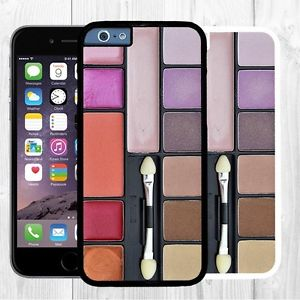
\includegraphics[width=25mm]{figures/eyeshadow-iphone-case.jpg}
                \caption{\textcolor{red}{{\bf Eyeshadow}} Palettes for \textcolor{red}{{\bf iPhone}} 6 case}
                \label{fig:eyeshadow-iphone-case}
        \end{subfigure}
              ~ %add desired spacing between images, e. g. ~, \quad, \qquad, \hfill etc.
          %(or a blank line to force the subfigure onto a new line)
        \begin{subfigure}[b]{0.3\textwidth}
		 \centering
                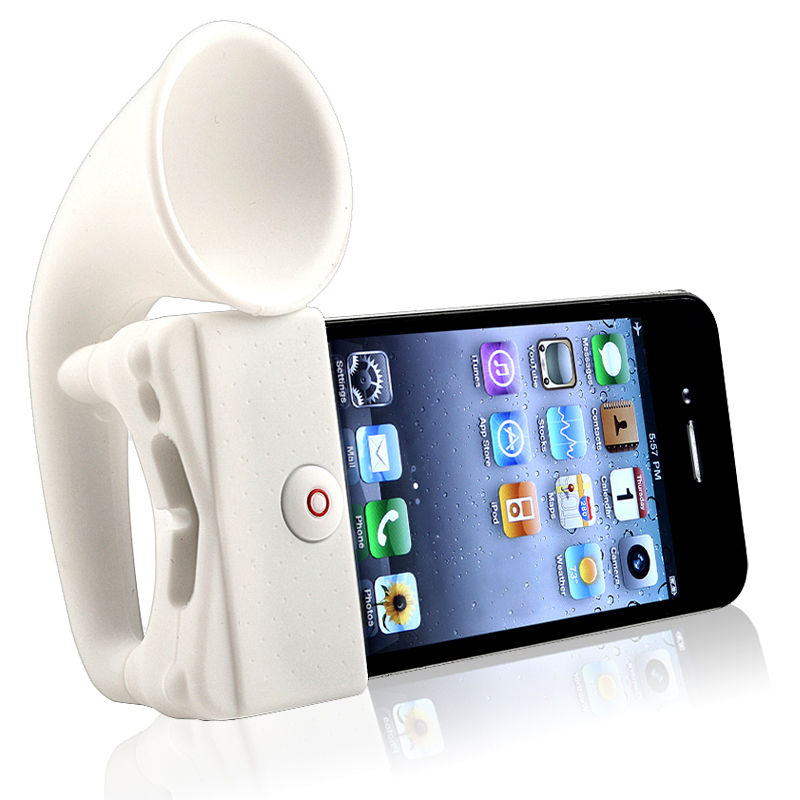
\includegraphics[width=25mm]{figures/horn-iphone-speaker.jpg}
\caption{White Silicone \textcolor{red}{{\bf Horn}} Stand Speaker for Apple \textcolor{red}{{\bf iPhone}} 4/ 4S}                \label{fig:zeppelin-speaker}
        \end{subfigure}
       ~ %add desired spacing between images, e. g. ~, \quad, \qquad, \hfill etc.
          %(or a blank line to force the subfigure onto a new line)
        \begin{subfigure}[b]{0.3\textwidth}
		 \centering
                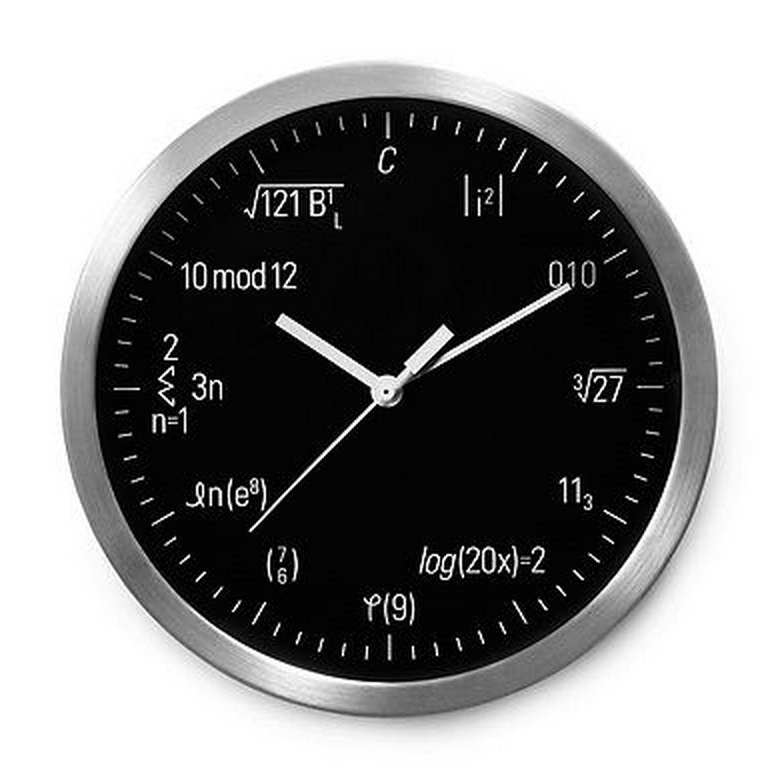
\includegraphics[width=30mm]{figures/geeky-clock.jpg}
\caption{\textcolor{red}{{\bf Equation}} Wall \textcolor{red}{{\bf Clock}} Gifts for Math Gurus}                \label{fig:geeky-clock}
        \end{subfigure}
       \caption{A collection of unique/interesting {\em eBay} products. Highlighted keywords demonstrate how the text associated with such products could span multiple diverse topics.}
       \label{fig:ebay-products}
\end{figure}

%%%%%%%%%%%%%%%%%%%%%%%%%%%%%%%%%%%%%%%%%%%%%%%%%%%%%%%%%%%%%
%%%%%%%%%%%%%%%%%%%%%%%%%%%%%%%%%%%%%%%%%%%%%%%%%%%%%%%%%%%%%
%%%%%%%%%%%%%%%%%%%%%%%%%%%%%%%%%%%%%%%%%%%%%%%%%%%%%%%%%%%%%

\section{Our Approach}
\label{sec:our-approach}

%\subsection{Word Representation}
%\label{sec:word-representation}

We assume a distributional representation for the words in the vocabulary (for a brief review
see~\cite{Turian10wordrepresentations}). A distributional representation over a vocabulary $V$ maps a word in the vocabulary to a 
probability distribution over a fixed domain $C$. Often we start by a co-occurrence matrix $\cM_{|V|\times|C|}$ where each row represents a co-occurrence of a word with domain
$C$. For example if we chose $C=V$ then we obtain the familiar {\sl word-to-word} co-occurrence representation which counts the number
of times two words co-occurred in a document corpus. Another choice would be to use the set of topics learned over a document
corpus by {\sl Latent Dirichlet Allocation} (LDA)~\cite{Blei:2003:LDA:944919.944937} as the domain. The rows of $A$
are then normalized in order to obtain a probability distribution over the topic domain. We will use the notation $P_w$ to represent
the probability distribution over the domain  given a word $w$. We also use the notation $W=\{w_1,...,w_k\}$ for a bag of word representation of a text snippet. Given a word distributional representation, $\cP_{W}=\{P_{w_1},...,P_{w_k}\}$ denotes the set of probability distributions over the words
in the text snippet.

%%%%%%%%%%%%%%%%%%%%%%%%%%%%%%%%%%%%%%%%%%%%%%%%%%%%%%%%%%%%%

\subsection{Information Diversity}
\label{sec:information-diversity}

Given a distributional representation over a vocabulary $V$ and a domain $C$ with $P_w$ giving a probability distribution of a
word $w$ over domain $C$, we can measure information diversity for a given text snippet $W=\{w_1,...,w_k\}$ and its
distributional representation $\cP_{W}=\{P_{w_1},...,P_{w_k}\}$ as follows:
\bed\label{importance}
Given a distribution $P_w$, its {\sl importance} with respect to a
prior distribution $P$ is defined as $D_w = D_{KL}(P_w\|P)$ where $D_{KL}(\|)$ denotes the
{\sl Kullback-Leibler} Divergence.
\eed
\bed\label{mixture}
Given a set of distributions $\cP_{W}=\{P_{w_1},...,P_{w_k}\}$ and a
prior $P$, we
define a mixture distribution $P_W=\sum_{i=1}^k d_{w_i} P_{w_i}$ where $d_{w_i}=\frac{D_{w_i}}{\sum D_{w_j}}$ are the normalized
importances.
\eed
Essentially, $P_W$ is the weighted average of the set $\cP_{W}$, where
the weights are chosen according to the importances. Next we
define the diversity measure:
\bed\label{diversity}
We define the Jensen-Shannon Information Diversity of a set of
distributions $\cP_W$ with respect to 
prior $P$ as $\mbox{JSD}_P(\cP_W)=\sum_{i=1}^k d_{w_i}D_{KL}(P_{w_i}\|P_W)$
where $d_{w_i}$ and $P_W$ are as in the previous definition.
\eed
This definition is closely related to the 
{\em general Jensen-Shannon Divergence}~\cite{FugledeTopsoe}. Another
interesting theoretical property of Jensen-Shannon Information
Diversity is that it can be interpreted as a generalization of Shannon
entropy as a population diversity measure, however we will not go
into this here any further. 

%%%%%%%%%%%%%%%%%%%%%%%%%%%%%%%%%%%%%%%%%%%%%%%%%%%%%%%%%%%%%

\subsection{Topic Diversity}
\label{sec:topic-diversity}

In order to apply this model to natural language we first need to build a distributional representation for words. One
natural choice for measuring the topic diversity is to use {\sl word-to-topic} distribution. We need to address the following problems:\\
{\bf (1) Building word to topic distribution}: We train an
LDA~\cite{Blei:2003:LDA:944919.944937} to build a topic model given a document corpus $\cC$. From this topic model we obtain the
word-topic matrix $\cM$ where $\cM_{ij}$ is the probability of $w_i$  given $j$-th topic which is given by the LDA model. By normalizing the rows of matrix $\cM$ we will obtain
a word-topic distribution, where the $i$-th row of the matrix gives the topic distribution for the word $w_i$ (note that word-to-topic distribution as described is not explicitly defined in the standard LDA model and our approach is one way to approximate it). We also use $T$ to denote the set of topics learned in the LDA model.\\
{\bf (2) Obtaining a prior topic distribution:} this is
required for computing the information diversity as described in Section~\ref{sec:information-diversity}. We obtain a prior
 topic distribution $P$ by computing the proportions of overall topic
 assignments. This corresponds to summing up matrix $\cM$ along its
 rows and then normalizing the resulting vector.\\
{\bf (3) Capturing topic similarity:} here we consider the problem first raised in~\cite{bache:2013}. When building a word-to-topic distribution model based on 
the word-to-topic co-occurrence matrix, the relationship among topics (i.e, topic similarity ) may be lost. For example, if a word $w$
has a topic distribution $P_w$ concentrated on some topic $t$, then it will
not necessarily peek at all other topics that are very similar to topic $t$. To address this problem, we first define a topic similarity matrix $\cS_{|T|\times|T|}$
where the $i^{th}$ row of $\cS$ gives the topic similarity vector for the $i^{th}$ topic (e.g., cosine similarity between topics~\cite{bache:2013}). We further assume that it is normalized 
and hence can be thought of as a topic similarity distribution. Using $\cS$ we obtain $\tilde{P}_w = P_w\cS^T$ which essentially diffuses the initial distribution to
one where  all topics similar to some topic $t$ are well represented. Similarly, we can use $\cS$ to to reflect the topic similarity in the prior distribution as $\tilde{P} = P\cS^T$.
In Section~\ref{sec:experiments} we will show how this
approach enhances the standard entropic measure of diversity.\\
{\bf (4) Sample size bias problem:}  note that 
when we normalize the rows of the matrix $\cM$ to obtain a distributional model, the normalization factor 
for every word is simply the word count. Thus for a word $w$ which occurs very rarely
in the entire corpus $\cC$, the topic distribution will be artificially skewed and is inaccurate simply because we do not have enough data points to estimate its true word-to-topic distribution.
Now, if for this corpus it happens that the prior topic distribution
is close to uniform, it will give a very high importance to the word
$w$ when measuring the information diversity as described in
Section~\ref{sec:information-diversity}.
One way to alleviate this
problem is to use the relative sample size (e.g., word count) to
smooth the distribution obtained by normalizing the rows of matrix
$\cM$. A natural choice for the smoothing distribution would in this
case be simply the prior distribution mentioned above. Applying {\em Laplace smoothing}
we get:
\begin{equation}
\widehat{P}_w=\frac{\alpha \tilde{P}+ \mu_w \tilde{P}_w}{\alpha+\mu_w}
\end{equation}
where $\mu_w$ is the frequency of word $w$ in D, and $P_w$ is the
topic assignment distribution obtained from the word-topic matrix,
while $\alpha$ is the parameter that specifies the strength of the
prior.\\
{\bf (5) Conditioning on context words:} we propose a final enhancement to the word-topic
distributions. Suppose, the set of words $W=\{w_1,...,w_k\}$
represents a text snippet that we want to analyze. The word $w_i$ has
a specific meaning inside of $W$, that can be significantly different
than its meaning out of context. Denote
$W_{\bar{i}}=W-\{w_i\}$ as the set of all words in $W$ except
$w_i$. By $P_{W_{\bar{i}}}$, we denote the mixture distribution for $W_{\bar{i}}$ (Definition \ref{mixture}) and we use $\tilde{P}_{W_{\bar{i}}}$ when it is smoothed using Laplace smoothing method. We
propose the following definition of context-dependent word-topic
distribution. 
\bed
Let $\tilde{P},\widehat{P}_{w_i}, \tilde{P}_{W_{\bar{i}}}$ be the topic prior, general
topic distribution for $w_i$, and the context distribution,
respectively. Then, the context-dependent distribution is
\begin{equation*}
P^{W_{\bar{i}}}_{w_i}(t)\propto \frac{\tilde{P}_{W_{\bar{i}}}(t)}{\tilde{P}(t)}\widehat{P}_{w_i}(t)
\end{equation*}
\eed
There is a probabilistic explanation that we have left out for 
lack of space. However this can be intuitively understood as follows:
we can think of $\frac{\tilde{P}_{W_{\bar{i}}}(t)}{\tilde{P}(t)}$ as a weight
that further reshapes the smoothed word-to-topic distribution $\widehat{P}_{w_i}(t)$
to take into account the context. In our experiments we also smooth this distribution
using {\em Laplacian} smoothing.

%%%%%%%%%%%%%%%%%%%%%%%%%%%%%%%%%%%%%%%%%%%%%%%%%%%%%%%%%%%%%
%%%%%%%%%%%%%%%%%%%%%%%%%%%%%%%%%%%%%%%%%%%%%%%%%%%%%%%%%%%%%
%%%%%%%%%%%%%%%%%%%%%%%%%%%%%%%%%%%%%%%%%%%%%%%%%%%%%%%%%%%%%

\section{Experiments}
\label{sec:experiments}

We used the following two datasets in our experiments: (1) Interesting iPhone cases:
for generating the ground truth data we hired workers from {\em Amazon Mechanical Turk (AMT)} to label a collection
of nearly 20,000 iPhone cases on {\em eBay}. The details of this step is beyond the scope of this paper, however we used insights from
interesting iPhone cases found on {\em Pinterest} and {\em eBay's} user behavior data in order to generate a balanced data-set. 
We then pulled our final dataset from the annotated by selecting only those instances where the annotators all labeled it as
positive (i.e., interesting) or negative (i.e., uninteresting). The final data-set consists of 2179 positive and 9770 negative instances for
a total of 11,949 instances. For each instance, the product title of
the corresponding {\em eBay} listing was used as the input. In this case we are
dealing with very short text snippets, usually 10 to 12 words each. To
train a topic model, we used a larger, more broader set of about
2 million product titles, grouped based on {\em eBay} categorical information into about 8,000
documents of approximately 200 titles each; (2) {\em NSF}
abstracts: for the second dataset we used a set of 61,902 National Science Foundation
Scholarship proposal abstracts (see~\cite{bache:2013} for more details) to evaluate how our diversity measure
compares to other methods on larger pieces of text. We used this set
for training a topic model, however to get labeled data, we had to
generate artificial examples, by randomly mixing pairs of abstracts that we
could expect to be either similar (small diversity) or very different
(high diversity) and labeling them accordingly. We generated 5,000 of
those examples with positive and negative labels evenly represented. For both datasets we used the Mallet LDA implementation and learned a topic model with $400$ topics.

We present two sets of results. First, we present
ROC curves comparing different entropic measures of topic diversity in an unsupervised setting 
(labeled data is only used for generating the curves). Figures~\ref{fig:phonecases-comparison} and \ref{fig:nsf-comparison}
compare our diversity metric using both topic similarity and context conditioning (labeled by {\em JSD-Sim-Con}) with a few baselines; namely LDA topic entropy, LDA topic entropy entropy using topic similarity (labeled by {\em Entropy-Sim}), {\em Rao diversity} (see~\cite{bache:2013} for details). In either case it can be observed that our diversity metric outperforms the other baselines with an AUC $0.73$ while the other measures give almost uninformative results. This can be explained for the {\em eBay} dataset since the text snippets are short. Thus the LDA may yield a poor topic inference for such short text and as a result all entropy measures using topic inference would perform also poorly. Figures~\ref{fig:phonecases-breakdown} and \ref{fig:nsf-breakdown} show the gains we obtain by application of the topic similarity and context conditioning techniques (steps 4, and 5) that we discussed in Section~\ref{sec:topic-diversity}. However, their degree of effects are different for each
dataset.  In the second set of results, we used the unnormalized vector of mixture topic
distribution (described in Definition~\ref{mixture}) computed over {\em eBay} product titles in a supervised classification setting. Table~\ref{tab:classification-results} compares the performance of the SVM classifier using our proposed mixture topic distribution as features to two different baselines, namely, SVM using {\em Latent Semantic Indexing (LSI)} features (by forming a document-term matrix and performing SVD), and a deep learning approach using the {\em recursive auto-encoders (RAE)} described in~\cite{Socher:2011:SRA:2145432.2145450}. These results are averaged over five different cross-validation splits of using $0.6$ for training and $0.4$ for testing. Our proposed approach shows a higher precision although marginally showing a higher accuracy compared to the baselines.

\begin{figure}
        \centering
        \begin{subfigure}[b]{0.24\textwidth}
                \centering
                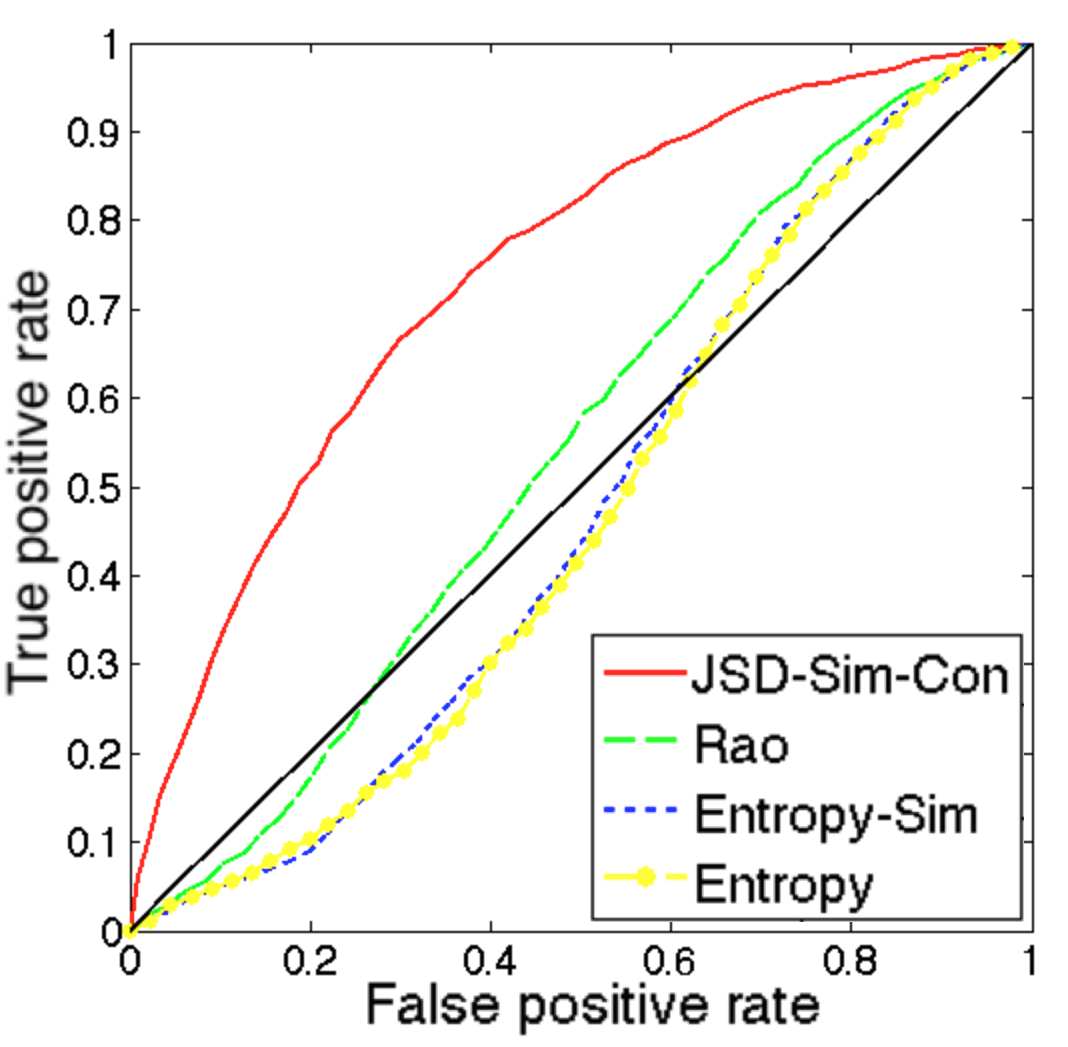
\includegraphics[width=36mm]{figures/phonecases-comparison-kopia.png}
               \caption{eBay (baseline)}
                \label{fig:phonecases-comparison}
        \end{subfigure}%\qquad
              ~ %add desired spacing between images, e. g. ~, \quad, \qquad, \hfill etc.
          %(or a blank line to force the subfigure onto a new line)
        \begin{subfigure}[b]{0.24\textwidth}
                \centering
                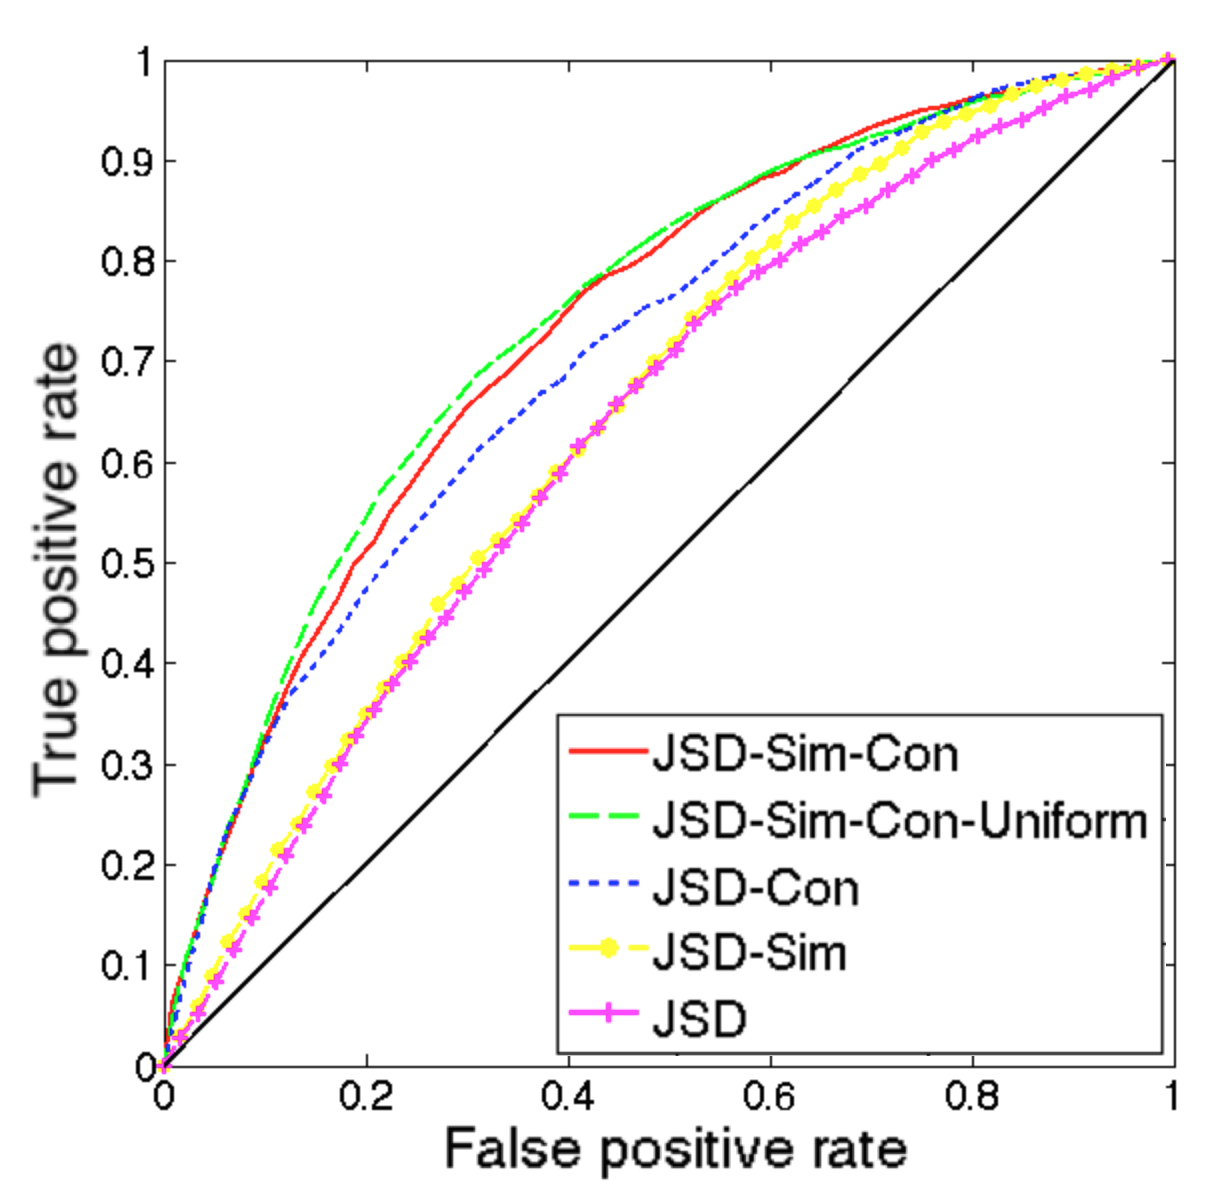
\includegraphics[width=36mm]{figures/phonecases-breakdown-kopia.png}
                \caption{eBay (JSD)}
                \label{fig:phonecases-breakdown}
        \end{subfigure}\nobreak
              ~ %add desired spacing between images, e. g. ~, \quad, \qquad, \hfill etc.
          %(or a blank line to force the subfigure onto a new line)
        \begin{subfigure}[b]{0.24\textwidth}
                \centering
                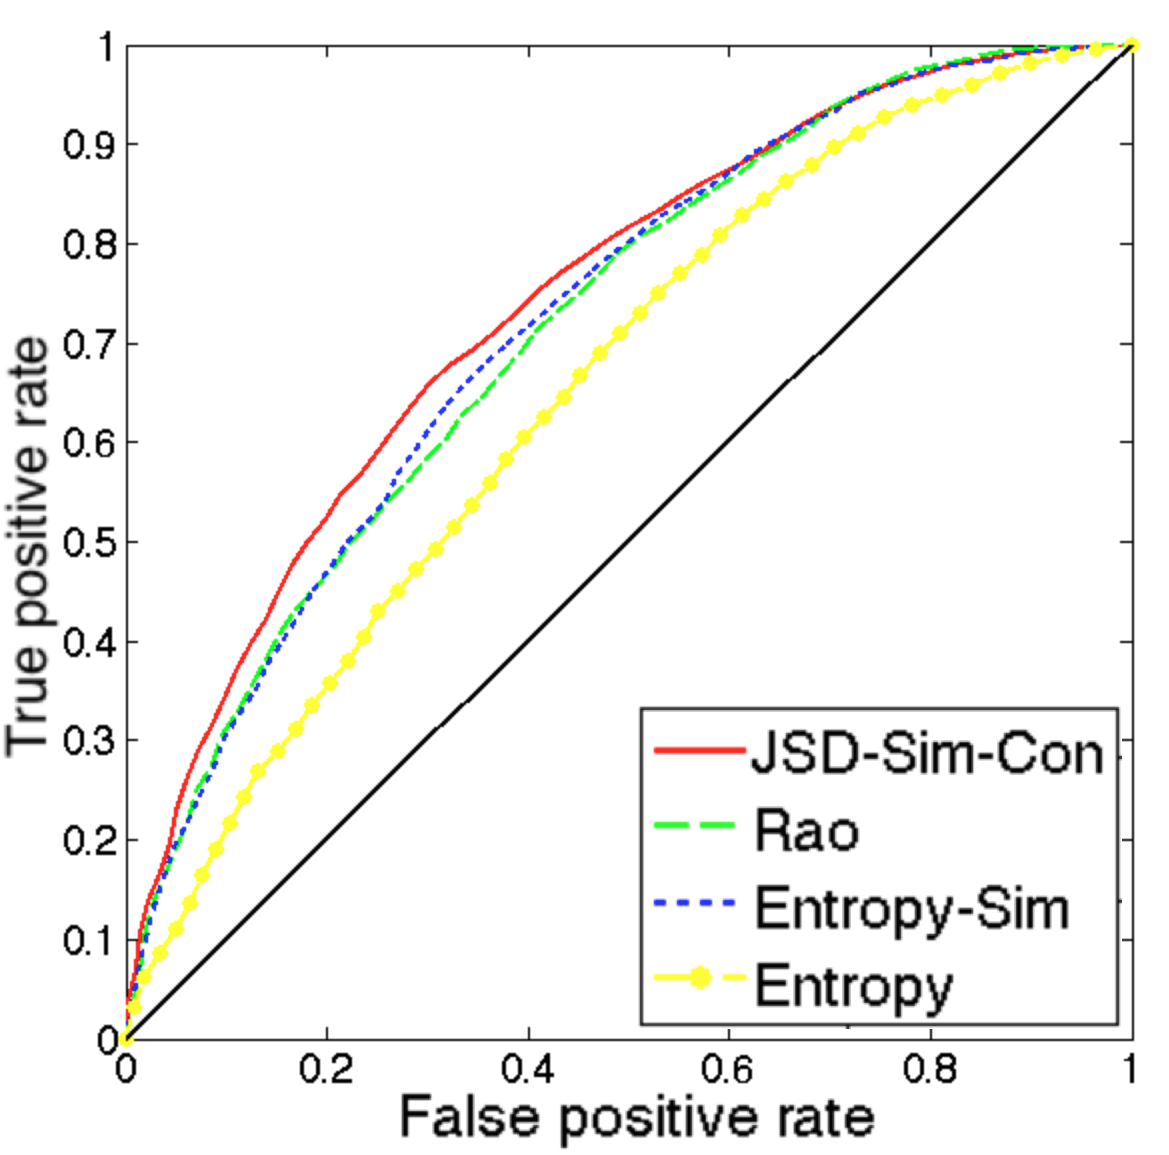
\includegraphics[width=36mm]{figures/nsf-comparison-kopia.png}
                \caption{NSF (baseline)}
                \label{fig:nsf-comparison}
        \end{subfigure}%\qquad
        ~ %add desired spacing between images, e. g. ~, \quad, \qquad, \hfill etc.
          %(or a blank line to force the subfigure onto a new line)
        \begin{subfigure}[b]{0.24\textwidth}
        	        \centering
                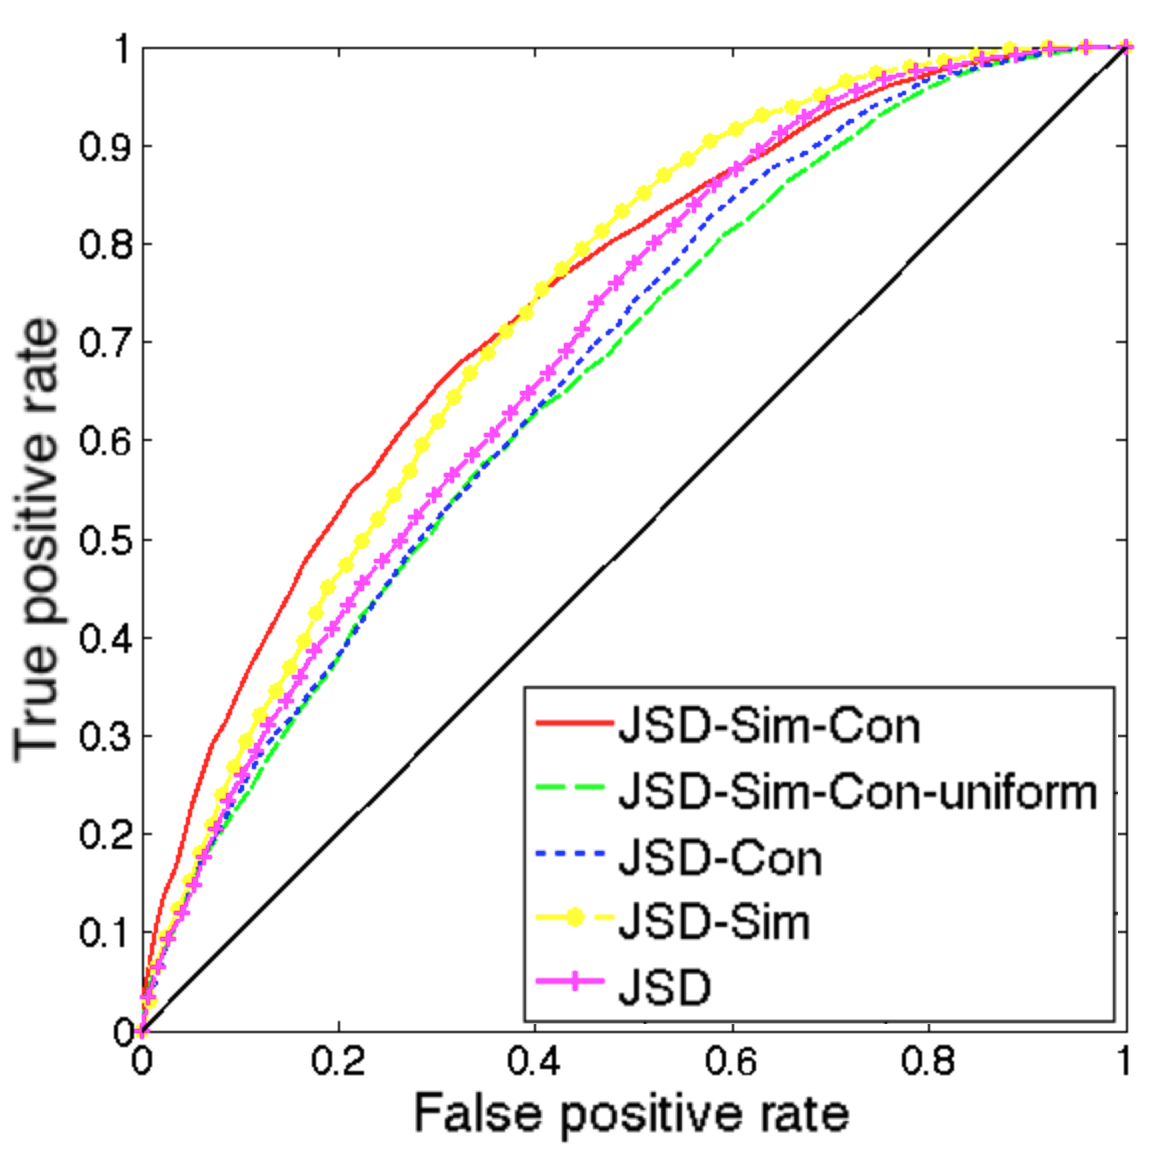
\includegraphics[width=36mm]{figures/nsf-breakdown-kopia.png}
               \caption{NSF (JSD)}
                \label{fig:nsf-breakdown}
        \end{subfigure}
       \caption{ROC curves presenting the results of experiments on
         the eBay dataset (a,b) and NSF proposal dataset (c,d). The
         comparison plots (a,c) show the results for our approach (JSD-Sim-Con)
         against other methods, while the breakdown plots (b,d)
         show different variations of our approach. }\label{fig:roc-curves}
\end{figure}


\begin{table}[t]
\caption{Classification results for the eBay dataset.}
\label{tab:classification-results}
\vspace{-4mm}
\begin{center}
\begin{tabular}{|l|c|c|c|c|}
\hline
&Precision & Recall & F1 & Accuracy
\\ \hline 
JSD Features         &$\mathbf{0.714}\pm 0.015$&$0.597\pm 0.016$&$0.650\pm
0.014$& $\mathbf{0.8828}\pm 0.0045$\\
RAE             &$0.676\pm 0.005$&$\mathbf{0.666}\pm 0.030$&$\mathbf{0.671}\pm
0.013$&$0.8809\pm 0.0020$ \\
SVD Features             &$0.676\pm 0.008$&$0.633\pm 0.017$&$0.654\pm
0.010$&$0.8778\pm 0.0027$\\
\hline
\end{tabular}
\end{center}
\end{table}

%%%%%%%%%%%%%%%%%%%%%%%%%%%%%%%%%%%%%%%%%%%%%%%%%%%%%%%%%%%%%
%%%%%%%%%%%%%%%%%%%%%%%%%%%%%%%%%%%%%%%%%%%%%%%%%%%%%%%%%%%%%
%%%%%%%%%%%%%%%%%%%%%%%%%%%%%%%%%%%%%%%%%%%%%%%%%%%%%%%%%%%%%

%\section{Conclusions}
%\label{sec:conclusions}

%%%%%%%%%%%%%%%%%%%%%%%%%%%%%%%%%%%%%%%%%%%%%%%%%%%%%%%%%%%%%
%%%%%%%%%%%%%%%%%%%%%%%%%%%%%%%%%%%%%%%%%%%%%%%%%%%%%%%%%%%%%
%%%%%%%%%%%%%%%%%%%%%%%%%%%%%%%%%%%%%%%%%%%%%%%%%%%%%%%%%%%%%




%%%%%%%%%%%%%%%%%%%%%%%%%%%%%%%%%%%%%%%%%%%%%%%%%%%%%%%%%%%%%
%%%%%%%%%%%%%%%%%%%%%%%%%%%%%%%%%%%%%%%%%%%%%%%%%%%%%%%%%%%%%
%%%%%%%%%%%%%%%%%%%%%%%%%%%%%%%%%%%%%%%%%%%%%%%%%%%%%%%%%%%%%

\bibliographystyle{plain}
\bibliography{nips2014}


\end{document}
